\documentclass[]{scrartcl}

\usepackage{listings}
\lstset{language=sql}  
\usepackage{hyperref}
\usepackage{graphicx}
\graphicspath{ {./images/} }

%opening
\title{sql100 v 1.0}
\author{Anthony BARBÉ}

\begin{document}
 

\date{}
\maketitle

\begin{center}
	Retrouver la dernière version de ce document sur : \\
	\url{https://github.com/AnthonyBARBE/sql100}
		
\end{center}


\newpage

\section{Énoncés}

\subsection{Afficher tout les titres de films sortis après 2004.}
	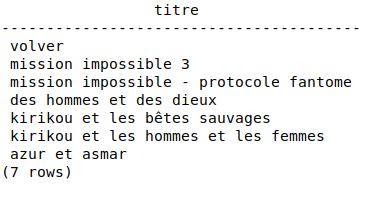
\includegraphics[scale=.5]{1}
	

\subsection{Traduire en français ce qu'affiche la requete suivante :}

\begin{lstlisting}[frame=single]  
	SELECT annee, titre 
	FROM film
	WHERE millesime>2004;
\end{lstlisting}

\subsection{Afficher la liste des acteurs du film 'volver'}
	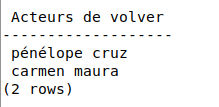
\includegraphics[scale=.5]{3}

\subsection{Qui a passé commande le 6 du mois ?}
	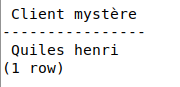
\includegraphics[scale=.5]{4}
	
\subsection{Combien y a-t-il de genres commençant par la lettre 'o' ?}
	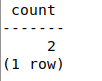
\includegraphics[scale=.5]{5}

\subsection{Afficher le nombre total de commande pour chaque ville, classé par ordre décroissant}
	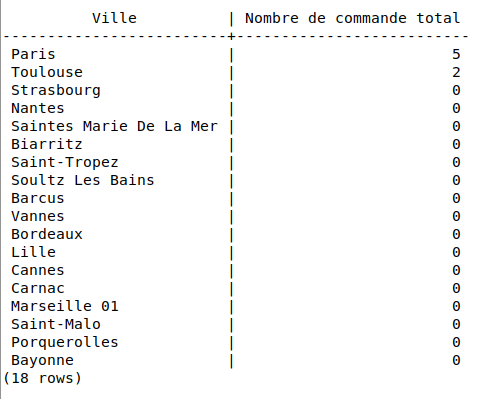
\includegraphics[scale=.5]{6}

\subsection{Récupérer les informations pour éditer les factures des trois dernières commandes (supposer des locations au format DVD et les prix de la table sont HT)}
	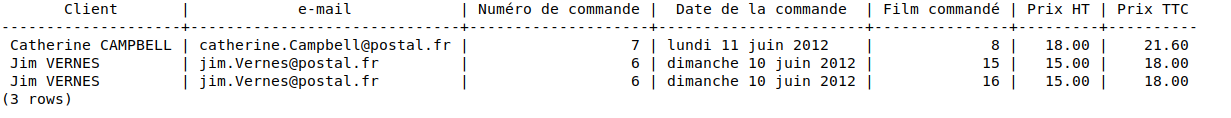
\includegraphics[scale=.4]{7}

\subsection{Afficher le dernier film commandé pour chaque client qui a un 'e' dans son prénom}
	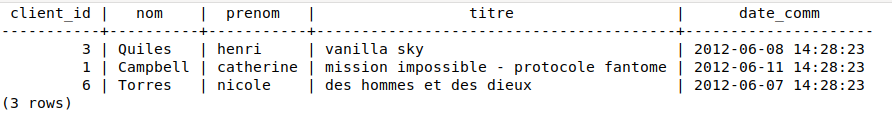
\includegraphics[scale=.5]{8}

\subsection{Pour chaque film, afficher la différence de prix d'une location en streaming par rapport à la moyenne du prix des locations en streaming}
	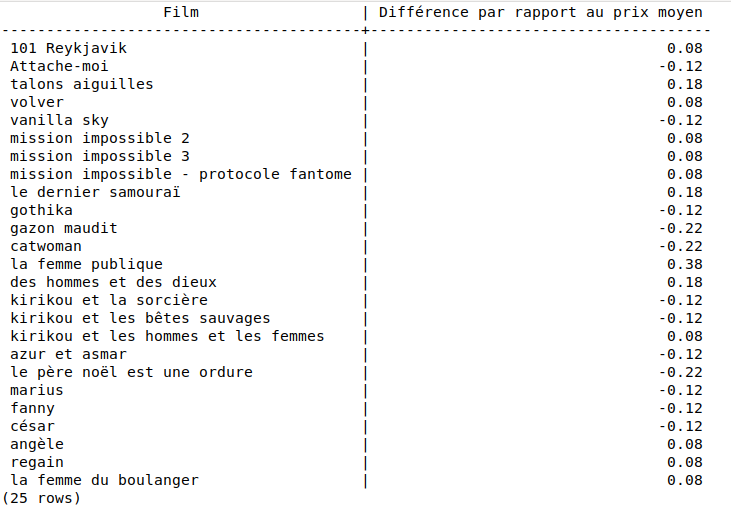
\includegraphics[scale=.5]{9}

\subsection{Quel acteur(s) jouai(en)t dans le premier film commandé ?}
	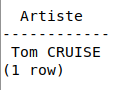
\includegraphics[scale=.5]{10}

\subsection{Traduire en français ce qu'affiche la requete suivante :}
  

\begin{lstlisting}[frame=single]  
	SELECT film.titre
	FROM film
	JOIN concerner ON film.film_id=concerner.film_id
	JOIN commande c ON concerner.commande_id=c.commande_id
	ORDER BY commande.date_comm DESC
	LIMIT 1;
\end{lstlisting}




\end{document}
